\documentclass{article}

% if you need to pass options to natbib, use, e.g.:
%     \PassOptionsToPackage{numbers, compress}{natbib}
% before loading neurips_2021

% ready for submission
\PassOptionsToPackage{numbers, compress}{natbib}
\usepackage[final]{neurips_2021}
\bibliographystyle{abbrvnat}


% to compile a preprint version, e.g., for submission to arXiv, add add the
% [preprint] option:
%     \usepackage[preprint]{neurips_2021}

% to compile a camera-ready version, add the [final] option, e.g.:
%     \usepackage[final]{neurips_2021}

% to avoid loading the natbib package, add option nonatbib:
%    \usepackage[nonatbib]{neurips_2021}

\usepackage[utf8]{inputenc} % allow utf-8 input
\usepackage[T1]{fontenc}    % use 8-bit T1 fonts
\usepackage{hyperref}       % hyperlinks
\usepackage{url}            % simple URL typesetting
\usepackage{booktabs}       % professional-quality tables
\usepackage{amsfonts}       % blackboard math symbols
\usepackage{nicefrac}       % compact symbols for 1/2, etc.
\usepackage{microtype}      % microtypography
\usepackage{xcolor}         % colors
\usepackage{graphicx}       % images
\usepackage{amsmath}

\title{Reinforcement Learning with Deep Q-Learning}

% The \author macro works with any number of authors. There are two commands
% used to separate the names and addresses of multiple authors: \And and \AND.
%
% Using \And between authors leaves it to LaTeX to determine where to break the
% lines. Using \AND forces a line break at that point. So, if LaTeX puts 3 of 4
% authors names on the first line, and the last on the second line, try using
% \AND instead of \And before the third author name.

\author{%
  Álvaro López Caro \\
  Universitat de Barcelona
  \And
  Vladislav Nikolov Vasilev \\
  Universitat de Barcelona
%   David S.~Hippocampus\thanks{Use footnote for providing further information
%     about author (webpage, alternative address)---\emph{not} for acknowledging
%     funding agencies.} \\
%   Department of Computer Science\\
%   Cranberry-Lemon University\\
%   Pittsburgh, PA 15213 \\
%   \texttt{hippo@cs.cranberry-lemon.edu} \\
  % examples of more authors
  % \And
  % Coauthor \\
  % Affiliation \\
  % Address \\
  % \texttt{email} \\
  % \AND
  % Coauthor \\
  % Affiliation \\
  % Address \\
  % \texttt{email} \\
  % \And
  % Coauthor \\
  % Affiliation \\
  % Address \\
  % \texttt{email} \\
  % \And
  % Coauthor \\
  % Affiliation \\
  % Address \\
  % \texttt{email} \\
}

\begin{document}

\maketitle

\begin{abstract}
  Reinforcement learning has become a very trendy topic in the machine learning
  field during the last couple of years due to its recent successes. It has allowed
  agents to learn to play many different games to the point of even defeating world
  champions, like AlphaGo did in 2016. Also, it is currently being applied to create
  self-driving cars. In this paper, we present the foundations of reinforcement learning and
  introduce one of the first successful deep learning-based approaches: Deep Q-Learning.
\end{abstract}

\section{Introduction}

When we think about the nature of learning, the idea that we learn by interacting with our
environment is the first to come to our mind. Throughout our lives, such interactions
(without the need of teachers or third agents) are undoubtedly a major source of knowledge about
our environment and about ourselves.

Indeed, learning from interaction is a foundational idea underlying nearly all theories of
learning and intelligence. \textbf{Reinforcement learning} is learning what to do (how to map
situations to actions) so as to maximize a numerical reward signal. The learner is not told
which actions to take, but instead must discover which actions yield the most reward by
trying them. In the most interesting and challenging cases, actions may affect not only
the immediate reward but also the next situation and, through that, all subsequent rewards.

In other words, let us think of an example of its application such as a master chess player
making a move. The choice is informed both by planning/anticipation and by immediate and intuitive
judgements of the desirability of particular positions and moves. In this or in any other example we
can come off with, they all involve \textbf{interaction} between an active decision-making agent and
its environment, within which the agent seeks to achieve a \textbf{goal} despite \textbf{uncertainty}
about its environment. The agent’s actions are permitted to affect the future state of the environment
(e.g., the next chess position), thereby affecting the actions and opportunities
available to the agent at later times. Correct choice requires taking into account indirect,
delayed consequences of actions, and thus may require foresight or planning.
At the same time, in any example given, the effects of actions cannot be fully predicted;
thus the agent must monitor its environment frequently and react appropriately. In any case,
the agent can use its experience to improve its performance over time.

In summary, reinforcement learning is a computational approach to understanding and automating
goal-directed learning and decision making. It is distinguished from other computational
approaches by its emphasis on learning by an agent from direct interaction with its
environment, without requiring exemplary supervision or complete models of the environment.
In interactive problems it is often impractical to obtain examples of desired behavior that are
both correct and representative of all the situations in which the agent has to act. In uncharted
territory—where one would expect learning to be most beneficial—an agent must be able to learn from
its own experience. In this way, reinforcement learning is different from supervised learning, the
kind of learning studied in most current research in the field of machine learning where we learn
from a training set of labeled examples provided by a knowledgeable external supervisor.

In the next section of this paper we are going to introduce the necessary background to understand
the different elements of reinforcement learning. We are also going to briefly discuss Q-Learning,
which is one of the fundamental algorithms in the area. After that, we are going to present
the recent advances in the field. Finally, we would like to introduce Deep Q-Learning, one
of the first deep learning-based algorithms used in the area that supposed a real breakthrough
due to the results that it offered.

\section{Background}

Reinforcement learning is the first field to seriously address the computational issues that arise
when learning from interaction with an environment in order to achieve long-term goals. It uses the
formal framework of Markov decision processes (MDPs) to define the interaction between a learning
\emph{agent} (the main actor) and its \emph{environment} (what the agent interacts with)
in terms of states, actions, and rewards. Figure \ref{fig:rl-interaction} illustrates how the
agent-environment interaction works. In MDPs, the transition between states is given
by a probability distribution $P(s' | s, a)$, where $s'$ is the next state, $s$ is the
current state, and $a$ is the selected action. This implies that the transitions
between states only depend on the most recent state and action. Basically, each state within an
environment is a consequence of all its previous states but storing all this information will become
infeasible, even for short \emph{episodes} (anything and everything that happens between the first state
and the last or terminal state within the environment). This is the reason that leads us to assume that
each state follows a Markov property, i.e., each state depends solely on the previous state and the
transition from that state to the current state.

\begin{figure}[h]
    \centering
    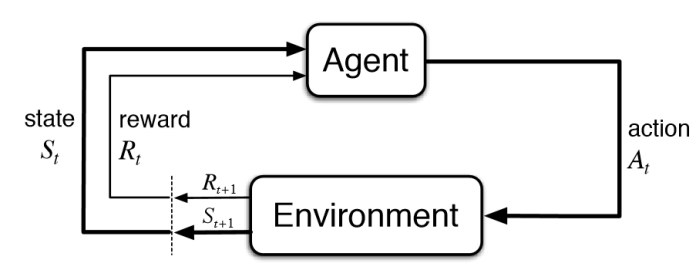
\includegraphics[width=0.7\textwidth]{img/reinforcement-learning-interaction.jpg}
    \caption{The agent-environment interaction in a Markov decision process.
    Original source: \cite{Sutton1998}.}
    \label{fig:rl-interaction}
\end{figure}

Beyond agent and environment, a reinforcement learning system has 4 subelements:

\begin{itemize}
    \item A \textbf{policy} that defines the learning agent’s way of behaving at a given time. Roughly
    speaking, a policy is a mapping from perceived states of the environment to actions to be taken
    when in those states. It can be stochastic and varies from a simple function to a search process.
    \item A \textbf{reward signal} defines the goal of a reinforcement learning problem. On each time
    step, the environment sends to the reinforcement learning agent a single number called
    the reward. The agent’s sole objective is to maximize the total reward it receives over
    the long run. The reward signal is the primary basis for altering the policy. In general, reward
    signals may be stochastic functions of the state of the environment and the actions taken.
    \item Whereas the reward signal indicates what is good in an immediate sense, a \textbf{value
    function} specifies what is good in the long run. Roughly speaking, the value of a state is
    the total amount of reward an agent can expect to accumulate over the future, starting
    from that state. Whereas rewards determine the immediate, intrinsic desirability of
    environmental states, values indicate the long-term desirability of states after taking into
    account the states that are likely to follow and the rewards available in those states. We
    seek actions that bring about states of highest value, not highest reward, because these
    actions obtain the greatest amount of reward for us over the long run. Unfortunately, it
    is much harder to determine values than it is to determine rewards.
    \item The fourth and final element of some reinforcement learning systems is a \textbf{model of
    the environment}. This is something that mimics the behavior of the environment, or
    more generally, that allows inferences to be made about how the environment will behave. Models are
    used for planning ahead but they are optional and some reinforcement learning algorithms are just
    based on trial-and-error learning as a way to change policies. Algorithms that try to learn
    a model of the environment are called \textbf{model-based} algorithms, whereas the ones that
    learn from trial-and-error are called \textbf{model-free} algorithms.
\end{itemize}

\subsection{Q-Learning}

Q-Learning is one of the most important reinforcement learning algorithms and is the foundation of many
of the modern techniques. It is a model-free algorithm and is based on \emph{Temporal Difference}
learning.

The algorithm tries to estimate the state-action values, also called Quality Values or \emph{Q-Values},
in order to find an optimal policy $\pi$. A Q-Value of a state-action pair $(s, a)$ is the expected
reward for choosing action $a$ in the state $s$ assuming that the agent acts optimally thereafter.
The algorithm constructs a table for each state-action pair which contains the estimations of the
Q-Values and it is updated as the agent explores the environment. To do this, it uses a dynamical
programming algorithm which updates the table using the following rule:

\begin{equation}
\label{bellman}
      Q_{t+1}(s_t, a_t) \leftarrow Q_t(s_t, a_t) + \alpha \left[ r_{t+1} + \gamma \max_{a} Q(s_{t+1}, a) - Q(s_t, a_t) \right]
\end{equation}


where $Q_{t+1}(s_t, a_t)$ is the new estimate, $Q_t(s_t, a_t)$ is the old one, $\alpha$ is the
learning rate, $r_t$ is the reward, $\gamma$ is the \emph{discount factor} and $\max_{a} Q(s_{t+1})$
is the estimate of the optimal future value. Usually, the learning rate $\alpha$ is a small value
between 0 and 1. The discount factor $\gamma$ is a number between 0 and 1, and it is related to how
important future rewards are compared to immediate rewards. The greater the value is, the more
importance is given to future rewards. Analogously, if its value is close to 0, then future rewards
are considered as not as important as immediate rewards. Normally, the value of $\gamma$ is set
to be close to 1 so that future rewards receive some importance when computing the estimations of the
Q-Values.

Although Q-Learning has been successfully applied to some problems, it presents some inherent flaws.
The first one is that as the number of states, the number of actions or both grow large, the problem
becomes intractable due to the amount of memory that it requires to store the table. Another one
is that it is prone to overestimate the Q-Values because it uses the $\max$ operator both to
evaluate and select the actions. This overestimation may lead to learning policies that are far
from the optimal, and therefore are of low quality.

\section{Related work}

During the years, many authors have made new proposals related to Q-Learning. One of this
contributions is Double Q-Learning \cite{NIPS2010_091d584f} (Álvaro), which addresses
the overestimation problem by learning two different Q-functions that are used to evaluate and
select the actions. These functions can be used interchangeably and they are updated randomly.
In general, the policies obtained from using this method are better than the ones obtained using
Q-Learning.

The advances in deep learning, especially in computer vision with the use of convolutional neural
networks, allowed to extract high-level features from raw sensory data. This served as a starting
point for the first successful deep learning-based proposal in reinforcement learning, which supposed
a real breakthrough in the area, and is none other than Deep Q-Learning
\cite{DeepMindAtari2013, mnih2015humanlevel} (Álvaro). In it, the authors proposed
a neural network architecture which they called \emph{Deep Q-Network} (DQN) that learned to predict
the Q-Values given the states as inputs. This addresses directly the intractability problem in
environments with a large number of states/actions, because the table was no longer needed.
The model was tested on different Atari 2600 games and showed state-of-the-art results in almost all
of them.

Many authors have put great endeavor in further improving Deep Q-Learning. One of these proposals
is Double DQN (Double DQN) \cite{DeepMindDDQN2015} (Vladislav), which is based on the same principles
as Double Q-Learning. It was observed that Deep Q-Learning was also prone to overestimate the Q-Values
due to the fact that it used the target network to both evaluate and select the actions. The proposal
in this case was to use the online model to select the best action and the target model to evaluate
it.

Another proposal is Dueling DQN (DDQN) \cite{DeepMindDueling} (Vladislav). In it, the authors showed that
the Q-Value for a state-action pair can be decoupled as $Q(s, a) = V(s) + A(s, a)$, where $V(s)$ is
the value of the state $s$ and $A(s, a)$ is the \emph{advantage} of taking action $a$ over the rest
of actions in state $s$. They proposed a network architecture called \emph{dueling architecture} in
which there is a shared convolutional part followed by two streams that estimate the value of the state
and the advantage separately and then aggregate these estimations in a special way to produce the actual
Q-Value estimations. This allows to learn both values separately and to learn which states are
valuable without having to learn the effects of each action for each state, which is particularly useful
in those states in which the actions do not impact the environment in any relevant way.

Finally, there was an attempt to combine several of the before mentioned techniques and some more into
a single agent called Rainbow \cite{DeepMindRainbow} (Vladislav). It was shown that by combining
the different techniques the agent was able to outperform all of the previous individual approaches
and to provide state-of-the-art results.

\section{Deep Q-Learning}

Q-Learning is a simple and powerful algorithm to create a cheat sheet for the agent to figure out which
action to perform. But a problem arises when this sheet is too long since we can work with environments
with thousands of states and hundreds of actions available per state. This leaves us with a table that
quickly becomes unmanageable. The amount of memory required to save and update the table would increase as
the number of states increases and the amount of time required to explore each state in order to create
the required table would be too much.

To solve this problem, DeepMind came with an algorithm that led to its acquisition by Google for 500
million dollars, the idea behind it being no other than using neural networks in order to approximate the
Q-values. Its original proposal published in Nature \cite{mnih2015humanlevel} constituted the first main
qualitative step in the use of deep learning in reinforcement learning settings. It used the advances in
DNN training to develop a novel artificial agent, termed a \textbf{Deep Q-Network} (DQN), that was able to
learn successful policies directly from high-dimensional sensory inputs using end-to-end reinforcement
learning. This agent was tested in the exciting and challenging environment of classic Atari 2600 games.
The Deep Q-Network agent, receiving only the pixels and the game score as inputs, was able to surpass the
performance of all previous algorithms and achieve a level comparable to that of a professional human games
tester across a set of 49 games, using the same algorithm, network architecture and hyperparameters. This
work bridges the division between high-dimensional sensory inputs and actions, resulting in the first
artificial agent capable of learning to excel at a diverse array of challenging tasks.

Before jumping into the details of the Deep Q-Learning algorithm that was used to achieve human-level
level performance in Atari games, let us clarify some of the underlying concepts involved in Deep
Q-Learning. For the reasons that we already mentioned, in Deep Q-Learning we use a neural network to
approximate the Q-Value function. The state is given as the input and the Q-Value of all possible actions
is generated as the output. In order to train the network it is used a \emph{replay memory} that
contains the last $N$ transitions of the game. Because using consecutive transitions to train the
network is inefficient since it introduces high correlations between the samples, the replay memory
is randomly sampled at each step of the training process generating a minibatch.

The proposed architecture of the DQN consists of three convolutional layers followed by two
fully connected layers with a single output for each valid action. The action that is going to be
executed next is the one that has the maximum Q-Value estimation. To train the network, the
loss function that the authors used is the mean squared error of the predicted Q-Value and the target
Q-Value using samples or minibatches of experience $(s, a, r, s') \sim \text{U}(D)$, drawn uniformly
at random from the replay memory. The loss can be expressed as follows:

\begin{equation}
  \label{eq:dqn-loss}
  L_i(\theta_i) = \mathbb{E}_{(s, a, r, s') \sim \text{U}(D)} \left[ \left( r + \gamma \max_{a'}Q(s', a';\theta_i^-) - Q(s, a; \theta_i) \right)^2 \right]
\end{equation}

Here there are two things to be noticed. The first one is that this loss resembles the Q-Learning
update rule (see equation \eqref{bellman}). The second one is that in equation \eqref{eq:dqn-loss}
appear two new elements: $\theta_i^-$ and $\theta_i$. The authors noticed that using the same network
to estimate the target values and select the actions made the training process unstable because
the target values are constantly changing when the weights of the network get updated. To overcome
this problem, they used two networks: one that is called the \emph{online model}, which is
updated at each iteration of the training loop, and one called \emph{target network} that is used
to estimate the target values. This second network gets a copy of the weights of the online model
every $C$ updates and stays frozen the rest of the time. Therefore, coming back to equation
\eqref{eq:dqn-loss}, $\theta_i^-$ refers to the weights of the target network, whereas $\theta_i$
refers to the weights of the online model.

With this in mind, let us present an overview of the steps followed in the Deep Q-Learning algorithm:

\begin{enumerate}
\item Working directly with raw Atari 2600 frames, which are 210x160
pixel images with a 128-color palette, can be demanding in terms of computation
and memory requirements. We apply a basic \textbf{preprocessing} step aimed at reducing
the input dimensionality and dealing with some artifacts of the Atari 2600 emulator. We then feed the game screen (state $s$) to our DQN, which will return the Q-values of all possible actions in the state.

\item Select an action using the \textbf{epsilon-greedy policy}: With the probability $\epsilon$, we select a random action $a$ and with probability $1-\epsilon$, we select an action that has a maximum Q-value.

\item Perform this action in a state $s$ and move to a new state $s’$ to receive a reward. This state $s’$ is the preprocessed image of the next game screen.

\item Save the transition in the replay memory.

\item Sample a random minibatch of transitions from the replay buffer and calculate the loss function which is just the mean squared difference between target Q and predicted Q with discount factor in play.

\item Perform \textbf{gradient descent} with respect to our actual network parameters in order to minimize this loss. It is often computationally expedient and stable to optimize the loss function by stochastic gradient descent.

\item After every $C$ iterations, copy our actual network weights to the target network weights.

\item Repeat these steps for $M$ number of episodes.

\end{enumerate}

The results achieved in the paper are shown below in figure \ref{games}. It can be seen that DQN
outperforms competing methods in almost all the games, and performs at a level that is broadly
comparable with or superior to a professional human games tester (that is, operationalized as a level
of 75\% or above) in the majority of games.

\pagebreak

\begin{figure}[t]
	\centering
	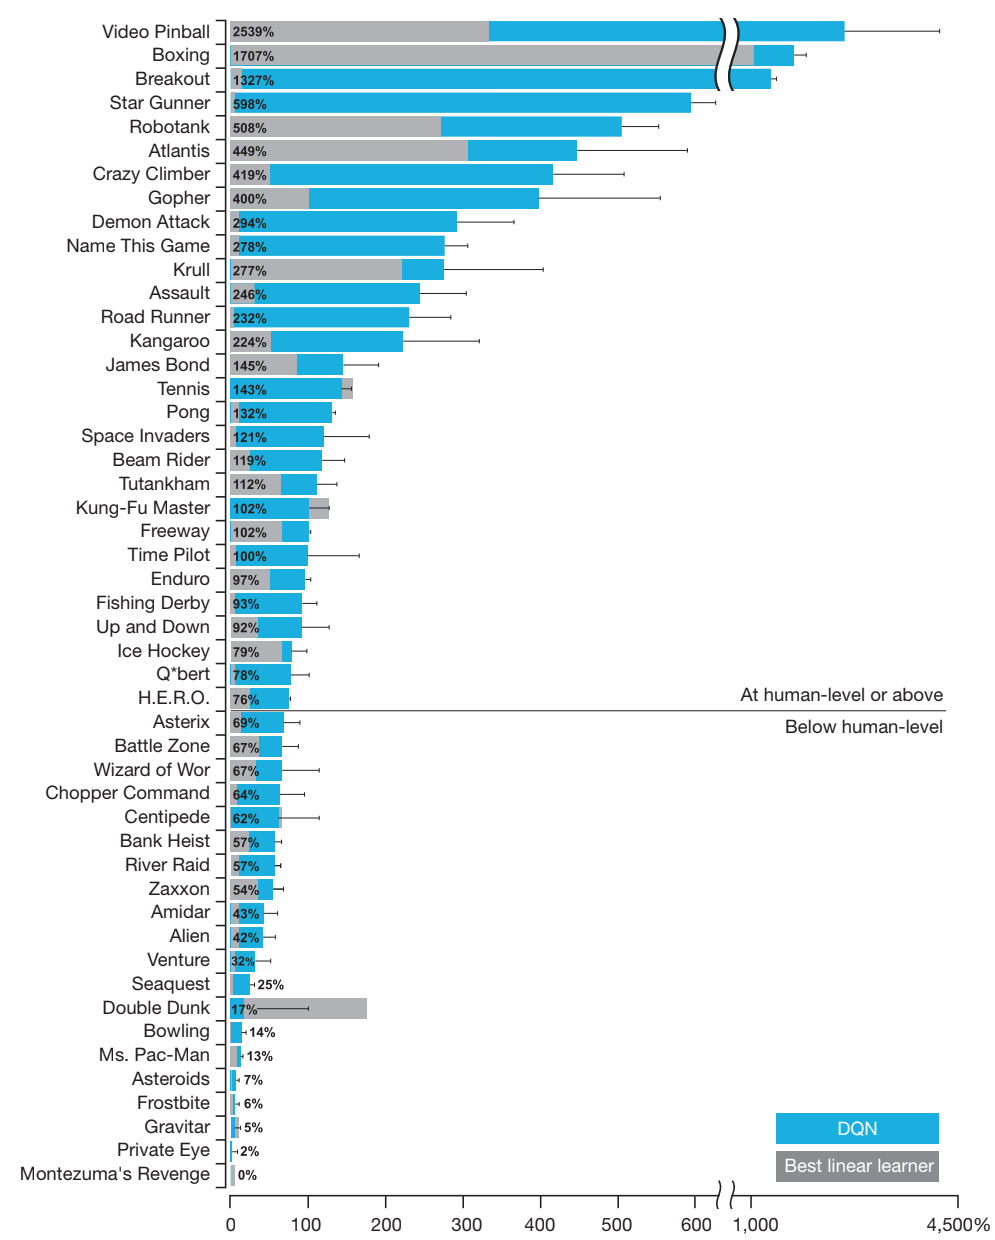
\includegraphics[width=13cm]{games.png}		
	\caption{Comparison of the DQN agent with the best reinforcement
learning methods in the literature at that particular moment. The performance of DQN is normalized
with respect to a professional human games tester (that is, 100\% level) and
random play (that is, 0\% level). Note that the normalized performance of DQN,
expressed as a percentage, is calculated as: $100 \cdot (\text{DQN score} - \text{random play
score}) / (\text{human score} - \text{random play score})$. \label{games}}
\end{figure}
\noindent


\nocite{*}
\bibliography{bibliography}


\end{document}